Các mẫu chiến lược phân tích nghiệp vụ kinh doanh sau đó đưa ra việc phân chia các thành phần và hiểu mối quan hệ của các thành phần đó. Từ đó, các mẫu chiến lược giúp xác định các thành phần quan trọng của hệ thống, đảm bảo kiến trúc phần mềm phản ánh đúng các yêu cầu kinh doanh. Từ việc phân chia hệ thống thành các thành phần nhỏ, chúng ta có thể tạo ra hệ thống mở rộng dễ dàng, phát triển linh hoạt theo nhu cầu kinh doanh.

Các mẫu chiến lược bao gồm:

\begin{itemize}

% các mục nhỏ ben dưới

% các mục nhỏ ben dưới

% các mục nhỏ ben dưới

% các mục nhỏ ben dưới

% các mục nhỏ ben dưới

% các mục nhỏ ben dưới

\item Muc1

\item Muc2

\item Muc1

\item Muc2

\item Muc1

\item Muc2

\item Muc1

\item Muc2

\end{itemize}

% nội dung trang lớn lên để hết giấy

% nội dung trang lớn lên để hết giấy

% nội dung trang lớn lên để hết giấy

% nội dung trang lớn lên để hết giấy

% nội dung trang lớn lên để hết giấy
 
\begin{figure}[H]

\centering

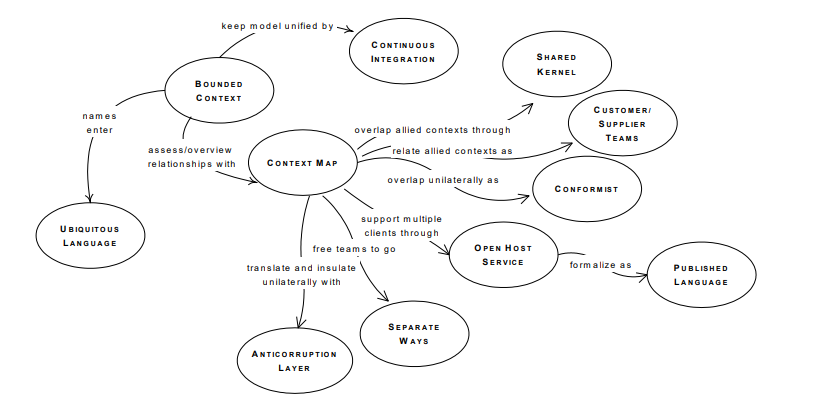
\includegraphics[scale = 0.9]{pictures/cac_mau_chien_luoc/temp.png}

\caption{Sơ đồ về các thành phần trong mô hình chiến lược}

\end{figure}

%!<! - - $ Vẽ lại sau: - - >

%!<! - - $ Vẽ lại sau: - - >

%!<! - - $ Vẽ lại sau: - - >

%!<! - - $ Vẽ lại sau: - - >

%!<! - - $ Vẽ lại sau: - - >

%!<! - - $ Vẽ lại sau: - - >

%!<! - - $ Vẽ lại sau: - - >

%!<! - - $ Vẽ lại sau: - - >

%!<! - - $ Vẽ lại sau: - - >

%!<! - - $ Vẽ lại sau: - - >

